\documentclass[10pt,onecolumn]{article}
% Package includes handled in a separate file
\title{VS265 Problem 16: PCA, ICA and Sparse-Coding}
\author{Archit Gupta}
\date{}
\input package-includes
\begin{document}
    \maketitle
    \vspace{-2em}
    \noindent\rule{\textwidth}{1.4pt}
    \vspace{1em}
    \begin{acronym}[challenge]
    \acro{PCA}[PCA]{Principal Component Analysis}
    \acro{ICA}[ICA]{Independent Component Analysis}
    \acro{IID}[IID]{Independent and Identically Distributed}
\end{acronym}


    \section{Problem description}
    \label{sec:problem_description}
    Over the years, scientists have debated on processing strategies employed by the brain to process the vast stream of sensory information in the natural world.
    Exploiting the underlying structure in the sensory information arising from natural scenarios is a recurring theme that has gained wide consensus.
    \ac{PCA}, \ac{ICA} and sparse-coding are some of the methods that allow us to find underlying or latent representations in data.
    Furthermore, under appropriate circumstances, all three methods can be applied for reducing the data dimensionality.

    In this challenge problem, we compare and contrast the three methods.
    First, in Section~\ref{sec:definitions} we look at the mathematical definitions of these modeling paradigms and comment on their similarities and difference.
    In Section~\ref{sec:examples_similarities}, we look at simplified datasets that illustrate the similarities of the three methods.
    Section~\ref{sec:examples_differences} illustrates how these methods differ, and discusses applications to real data.

    \section{Definitions}
    \label{sec:definitions}
    The models under discussion here assume that the underlying generative model is linear.
    In particular, the data, given by $\mathbf{x}\in\mathbb{R}^n$ arises from the model\footnote{We assume that the data lies in an n-dimensional vector space} given in Equation~\ref{eqn:generative_linear_model}.
    \begin{equation}
        \mathbf{x} = \mathbf{A}\mathbf{s} + \mathbf{n}
        \label{eqn:generative_linear_model}
    \end{equation}
    The matrix $\mathbf{A}$ has $n$ rows and $m$ columns with each column representing a basis vector.
    $\mathbf{x}$ can now be represented as a weighted sum of the basis vectors in $\mathbf{A}$.
    If we call the $m$ basis vectors $\mathbf{A_1}, \mathbf{A_2}, \dots, \mathbf{A_m}$, where $\mathbf{A_k}\in\mathbb{R}^n$, we are using a weighted combination $s_1\mathbf{A_1} + s_2\mathbf{A_2} + \dots, s_m\mathbf{A_m}$ to represent $\mathbf{x}$.
    The basis coefficients $s_1,s_2,\dots,s_m$ constitute the coefficient vector $\mathbf{s}\in\mathbb{R}^m$.
    Additionally, we incorporate $\mathbf{n}$ to model noise in measurement or modeling. 
    Typically, $\mathbf{n}$ is assumed to be comprised of \ac{IID} Gaussian random variables.
    We will look at how the three approaches \ac{PCA}, \ac{ICA} and sparse-coding find the model parameters $\mathbf{A}$ and $\mathbf{s}$.

    \subsection{\ac{PCA}}
    \label{sec:def_pca}
    \ac{PCA} gives us a complete basis of $n$ basis vectors, called the principal components.
    Because of the strict constraints on the \ac{PCA} solution, it is mathematically tractable and offers a lot of insight into various properties which can then be generalized to the other algorithms.
    In \ac{PCA}, we constrain the basis vectors $\mathbf{A_1},\mathbf{A_2},\dots,\mathbf{A_n}$ to be orthonormal, \textit{i.e.},
    \begin{equation}
        \mathbf{A_i}\cdot\mathbf{A_j} =
            \left\{
                \begin{array}{ll}
                    0 & \mbox{if } i\neq j \\
                    1 & \mbox{if } i = j
                \end{array}
            \right.
        \label{eqn:orthonormality_of_A}
    \end{equation}

    The basis vectors (which are now called principal components) being orthogonal results in the matrix $\mathbf{A}_{n\times n}$ being a unitary matrix.
    \begin{equation}
        \mathbf{A}^*\mathbf{A} = \mathbf{A}\mathbf{A}^* = \mathbf{I},
        \label{eqn:matrix_orthonormality}
    \end{equation}
    where $\mathbf{I}$ is the identity matrix of size $n$.
    Assuming that the data $\mathbf{x}$ is centered, the resultant matrix $\mathbf{A}$ can be found by diagonalizing the covariance matrix $\mathbf{X}\mathbf{X}^T$, where $\mathbf{X}$ is an $n\times{m}$ matrix comprised of the data entries $\mathbf{x}$ stacked along its columns.

    Since the covariance matrix is square and symmetric, it is always diagonalizable.
    Diagonalizing the covariance matrix gives us
    \begin{equation}
        \mathbf{X}\mathbf{X}^T = \mathbf{A}\mathbf{\Lambda} \mathbf{A}^*
        \label{eqn:matrix_diagonalization}
    \end{equation}
    The matrix $\mathbf{\Lambda}$ is vital for an understanding of \ac{PCA} as the diagonal entries represent the total amount of variance explained by the principal component.
    \begin{figure}[H]
        \centering
        \begin{tabular}{p{0.32\textwidth}p{0.32\textwidth}p{0.32\textwidth}}
            \sidesubfloat[]{\label{fig:faces_and_reconstruction}
                \centering
                \begin{tabular}{cc}
                    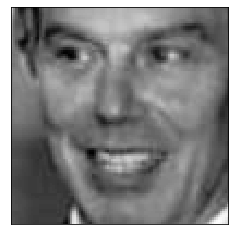
\includegraphics[width=0.4\linewidth]{figures/eigenfaces_example_1.png}&
                    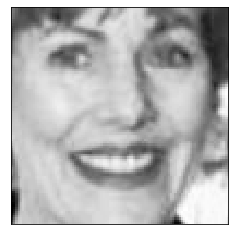
\includegraphics[width=0.4\linewidth]{figures/eigenfaces_example_2.png}\\
                    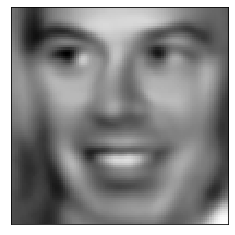
\includegraphics[width=0.4\linewidth]{figures/eigenfaces_recon_1.png}&
                    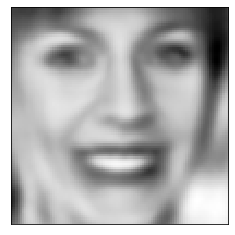
\includegraphics[width=0.4\linewidth]{figures/eigenfaces_recon_2.png}
                \end{tabular}
            }&
            \sidesubfloat[]{\label{fig:eigenfaces_explained_variance}
                \centering
                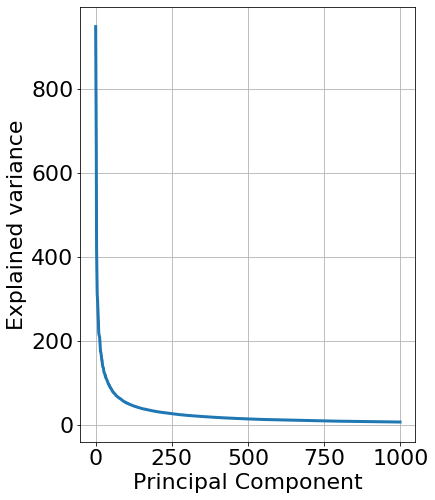
\includegraphics[height=0.9\linewidth]{figures/eigenfaces_explained_variance.png}
            }&
            \sidesubfloat[]{\label{fig:first_50_eigenfaces}
                \centering
                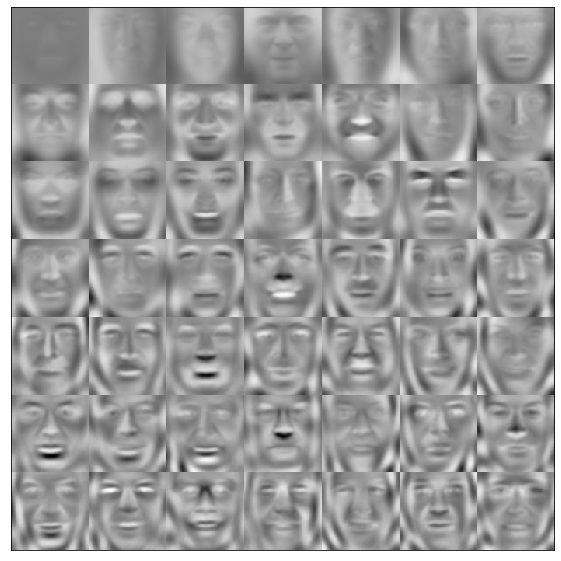
\includegraphics[width=0.8\linewidth]{figures/first_50_eigenfaces.png}
            }
        \end{tabular}
        \caption{\label{fig:applying_PCA_on_eigenfaces} Illustration of image compression with \ac{PCA}.
        \protect\subref{fig:faces_and_reconstruction} Example (Top) images of faces and their reconstruction (Bottom) using the first 100 of 13233 principal components.
        \protect\subref{fig:eigenfaces_explained_variance} Variance explained by each of the first 1000 principal components.
        \protect\subref{fig:first_50_eigenfaces} Top 50 eigenfaces (principal components).}
    \end{figure}
    Figure~\ref{fig:applying_PCA_on_eigenfaces} shows the application of \ac{PCA} to a set of images containing faces\footnote{dataset and code from the Summer 2020 iteration of EE16B taught at UC Berkeley}.
    In Figure~\ref{fig:eigenfaces_explained_variance}, we see that the total amount of explained variance drops rapidly.
    While the entire dataset is comprised of vectors in $n=13233$ dimensional space, the first $\sim100$ principal components explain most of the variance in data.
    The first $50$ principal components are shown in Figure~\ref{fig:first_50_eigenfaces} and images recostructed using only the first $100$ principal components are shown in Figure~\ref{fig:faces_and_reconstruction} (Top: Original, Bottom: Reconstructed).

    With this, we can list some of the important properties of \ac{PCA} that we will compare and contrast against the other methods.
    \begin{enumerate}
        \item The basis vectors and obtained from \ac{PCA} are complete and orthonormal.
        \item Different basis vectors explain different amounts of variance in the data - In some sense, they are not equally important.
        \item The weights (or variance explained) for different basis vectors drops rapidly in most natural datasets.
        \item Basis vectors are unique up to permutation and sign - This follows naturally from diagonalization not being unique.
            In practice, principal components are often arranged in a decreasing order of explained variance.
    \end{enumerate}

    \subsection{\ac{ICA}}
    \label{sec:def_ica}
    Similar to \ac{PCA}, \ac{ICA} produces a complete basis of $n$ basis vectors, or independent components.
    The underlying assumption for the data is that it is generated from a set of non-Gaussian sources that are statistically independent.
    While in \ac{PCA}, the basis vectors $\mathbf{A_1},\mathbf{A_2},\dots,\mathbf{A_m}$ are constrained to be orthonormal, in \ac{ICA}, this constraint is relaxed to $\mathbf{A_1},\mathbf{A_2},\dots,\mathbf{A_m}$ being linearly independent.
    Mathematically
    \begin{equation}
        \mathbf{A}\mathbf{s}\neq \mathbf{0}, \mbox{ for } \mathbf{s}\in\mathbb{R}^n-\mathbf{0}
        \label{eqn:defining_independence}
    \end{equation}
    Such a relaxation is more useful in practice, especially when we have prior information that $\mathbf{x}$ arises from a mixture of linearly-independent sources.
    Solving for the best solutions $\mathbf{A}$ and $\mathbf{s}$ is computationally expensive and several numerical solutions exist for finding model parameters that minimize the error~\cite{oja2006fastica,hyvarinen1999fast}.
    More importantly, the \ac{PCA} solution is a valid \ac{ICA} solution as well.

    \subsection{Sparse-Coding}
    \label{sec:def_sparse_coding}
    In sparse-coding, we usually find an over-complete basis or dictionary of vectors, $m>n$.
    The constraint changes to a maximization of sparsity of the coefficient vector $\mathbf{s}$.
    \begin{equation}
        \min_{\mathbf{A,s}}~\left\lVert\mathbf{s}\right\rVert_{0}, \mbox{ s.t. } \mathbf{x} = \mathbf{A}\mathbf{s} + \mathbf{n}
        \label{eqn:}
    \end{equation}

    For a fixed number of basis vectors ($m$), this often results in a trade-off between
    \begin{enumerate}
        \item Accurately modeling the data, i.e. reducing the error $\left\lVert\mathbf{e}_2\right\rVert^2 = \left\lVert\mathbf{x} - \mathbf{A}\mathbf{s}\right\rVert_2^2$, and
        \item The desired sparsity or $\left\lVert{\mathbf{s}}\right\rVert_0$, which is the typical number of non-zero coefficients required to express a data point $\mathbf{x}$.
    \end{enumerate}

    \section{Similar properties}
    \label{sec:examples_similarities}

    \begin{figure}[H]
        \centering
        \begin{tabular}{cc}
            \sidesubfloat[]{\label{fig:single_source_pca}
                \centering
                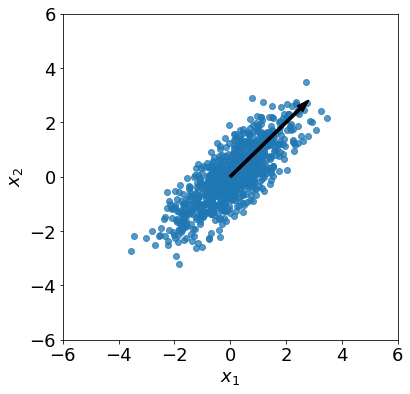
\includegraphics[width=0.25\linewidth]{figures/single_source_PCA.png}
            }&
            \sidesubfloat[]{\label{fig:two_orthogonal_sources}
                \centering
                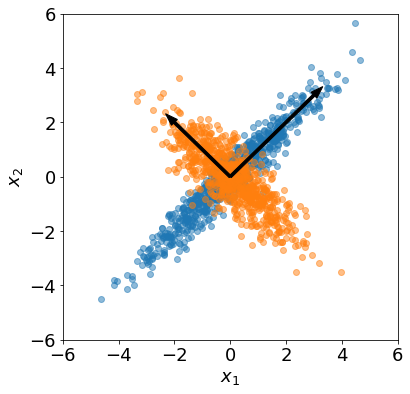
\includegraphics[width=0.25\linewidth]{figures/two_orthogonal_sources_PCA.png}
            }
            %\sidesubfloat[]{\label{fig:single_source_comp_PCA}
            %    \centering
            %    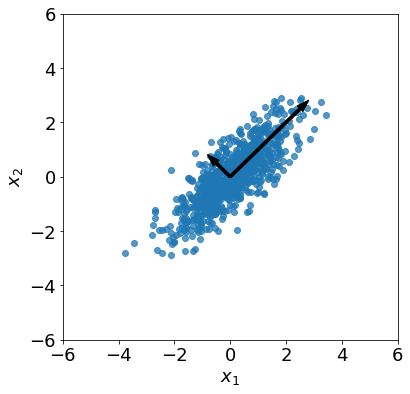
\includegraphics[width=0.25\linewidth]{figures/single_source_comp_PCA.png}
            %}&
            %\sidesubfloat[]{\label{fig:single_source_ICA}
            %    \centering
            %    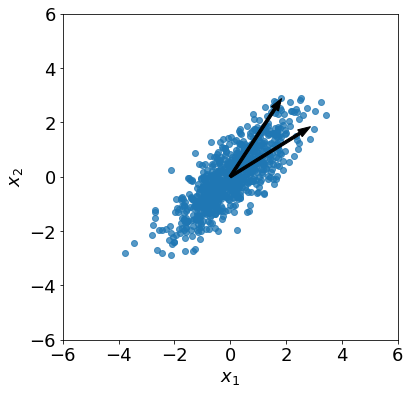
\includegraphics[width=0.25\linewidth]{figures/single_source_ICA.png}
            }
        \end{tabular}
        \caption{\label{fig:pca_ica_sparse_coding_on_perp_data} \ac{PCA} \texit{vs.} \ac{ICA} \textit{vs.} Sparse-Coding on data generated from orthogonal sources.}
    \end{figure}
    Figure~\ref{fig:pca_ica_sparse_coding_on_perp_data} shows data generated from a single Gaussian source.
    Our three methods, \ac{PCA}, \ac{ICA} and sparse-coding, when employed to find a single source in this data will all estimate the correct basis vector that generates this data (shown in Figure~\ref{fig:single_source_pca}).
    This direction, along the vector $\begin{bmatrix}1, 1\end{bmatrix}^T$, explains the most variance in the data  (\ac{PCA}), and is also the best choice for a sparse representation.

        Similarly, as shown in Figure~\ref{fig:two_orthogonal_sources}, if the data arises from two independent and orthogonal sources, all three methods, when restricted to finding 2 basis vectors find identical results.

    \section{Differences}
    \label{sec:examples_differences}

    While our methods produce similar results on the example datasets comprised of orthogonal sources shown in Section~\ref{sec:examples_similarities}, their differences appear when we relax this constraint on the sources and number of basis components.
    % For a single source, if we look for multiple independent components, we are likely to see a result shown in Figure~\ref{single_source_ICA}, where multiple basis components can better explain the data than a single one and additional constraints (like restricting the number of independent components) are needed to  get the correct basis.
    % \ac{PCA} and sparse-coding on the other hand, produce a result shown in Figure~\ref{fig:single_source_comp_PCA} since these two vectors maximize the variance, as well as representational sparsity.

    \begin{figure}[H]
        \centering
        \begin{tabular}{cc}
            \sidesubfloat[]{\label{fig:non_ortho_pca}
                \centering
                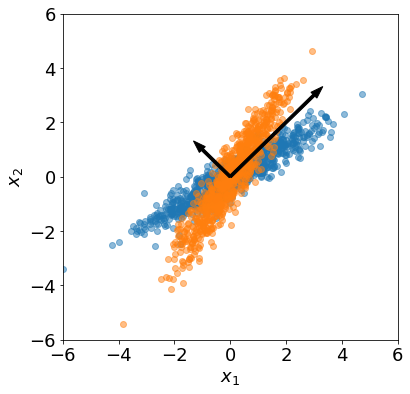
\includegraphics[width=0.25\linewidth]{figures/two_non_orthogonal_sources_pca.png}
            }&
            \sidesubfloat[]{\label{fig:non_ortho_ica}
                \centering
                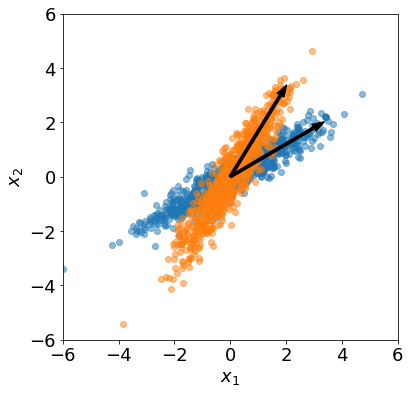
\includegraphics[width=0.25\linewidth]{figures/two_non_orthogonal_sources_ica.png}
            }
        \end{tabular}
        \caption{\label{fig:pca_ica_sparse_coding_on_non_perp_data} \ac{PCA} \texit{vs.} \ac{ICA} \textit{vs.} Sparse-Coding on data generated from non-orthogonal sources.}
    \end{figure}
    When looking at non-orthogonal sources, as can be seen in Figure~\ref{fig:non_ortho_pca}, the principal components find directions of maximal variance, whereas \ac{ICA} and sparse-coding in Figure~\ref{fig:non_ortho_ica} identify the sources which would lead to a sparser representation.

    \begin{figure}[H]
        \centering
        \begin{tabular}{ccc}
            \sidesubfloat[]{\label{fig:three_source_pca}
                \centering
                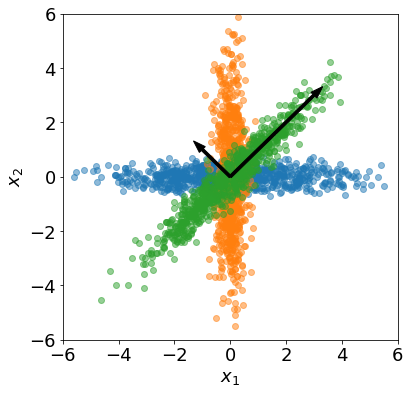
\includegraphics[width=0.25\linewidth]{figures/three_source_PCA.png}
            }&
            \sidesubfloat[]{\label{fig:three_source_ica}
                \centering
                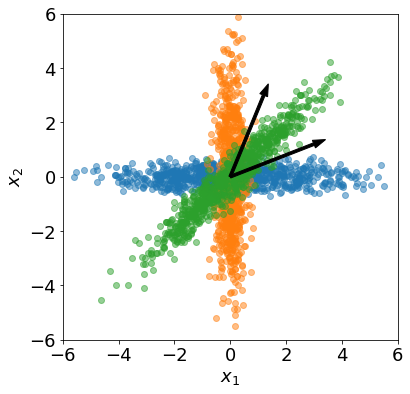
\includegraphics[width=0.25\linewidth]{figures/three_source_ICA.png}
            }&
            \sidesubfloat[]{\label{fig:three_source_sc}
                \centering
                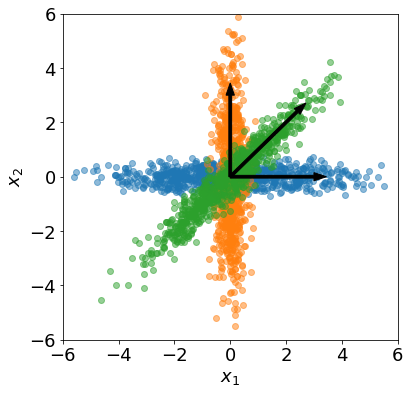
\includegraphics[width=0.25\linewidth]{figures/three_source_SC.png}
            }
        \end{tabular}
        \caption{\label{fig:pca_ica_sparse_coding_on_three_sources} \ac{PCA} \texit{vs.} \ac{ICA} \textit{vs.} Sparse-Coding on data generated from redundant sources.}
    \end{figure}
    When we have multiple, non-orthogonal sources, sparse-coding will identify all the sources for maximizing sparsity (Figure~\ref{fig:three_source_sc}).
    This is largely due to the flexibility afforded by an over-complete representation.
    Since \ac{PCA} and \ac{ICA} are restricted to find $n$ basis vectors, \ac{PCA} finds the directions of maximal variance (Figure~\ref{fig:three_source_pca}), whereas \ac{ICA} would find a set of linearly independent vectors that best explain the data (Figure~\ref{fig:three_source_ica}).

    When applied to data arising in natural scenarios, we see differences in the representational capabilities of these models as well.
    As seen in Figure~\ref{fig:first_50_eigenfaces} for a dataset of faces, the basis vectors resemble different features and frequency components of faces.
    When sparse-coding is applied to natural scenes~\cite{olshausen2004sparse}, we observe wavelet-like filters as the basis elements instead which points at another difference in these methods in practice.

    \section{Summary}
    \label{sec:summary}
    All the methods that we have discussed uncover latent structure in the data.
    As we saw in Figure~\ref{fig:applying_PCA_on_eigenfaces}, this structure can be used to reduce the data dimensionality.
    The basis components shown in Figure~\ref{fig:first_50_eigenfaces} reveal the underlying structure in these images.
    We also looked at simplified datasets comprised of independent sources and how the three methods compare on these.

    In~\cite{field1994goal}, the author discusses the role of sensory coding.
    Our brains constantly process a vast stream of sensory data.
    This data is highly structured and methods like \ac{PCA}, ac{ICA} and sparse-coding reveal the underlying structure in this data.
    They also offer an opportunity to validate computational theories about information processing in the brain.
    One such theory, argued in~\cite{field1994goal} for example is that the role of sensory coding is to translate the redundancy in sensory information to redundancy in neural coding.
    At the same time \ac{PCA} and \ac{ICA} offer an organizational principal for compression in the brain because of limited bandwidths.

    \setlength{\bibsep}{2pt}
    \bibliographystyle{unsrt}
    \footnotesize
    \bibliography{citations.bib}
\end{document}
